%% example for producing articles in MVA format using LaTeX.
%% written by Takeshi MASUDA, Electrotechnical Laboratory, Japan in May 1996.
%% modified by KAGESAWA Masataka, OKAZAKI Shin'ichro, YASUMOTO Mamoru.
%% last modified by Masaki Onishi, AIST, in Nov 2012.
%% use at your own risk.

\documentclass{mva_style}
\usepackage{graphicx}

\finalcopy %Uncomment this line for the Camera-Ready Manuscript

\begin{document}
\title{Agustin Castillo Munguia --- Paper Submissions (Tex format) ---}

\author{
  First Author Name\\
  Affiliation1\\
  Address1\\
  {\tt e-mail address1}\\
  \and
  Second Author Name\\
  Affiliation2\\
  Address2\\
  {\tt e-mail address2}\\
}

\maketitle


\section*{\centering Abstract}
\textit{
  This sheet is an example of how your manuscript should look like. 
  To ensure a uniform appearance in the proceedings, 
  authors are requested to conform to the directions below. 
  The camera-ready manuscripts for accepted papers 
  will appear in the proceedings in the same size and style.
}

\section{General Instructions}
\subsection{Note for authors}

The following review policy is adopted.

\begin{itemize}
  \item[(1)] Full paper should be submitted for review. 
    The paper must follow this instruction.
  \item[(2)] Page limit is 4 pages, excluding
    references. Papers should be
    printable on A4 paper.
  \item[(3)] MVA review is double-blind. 
    All papers submitted for review must maintain anonymity.
  \item[(4)] MVA 2023 does not consider a paper on arXiv.org as a dual submission.
\end{itemize}

\begin{description}  
\item[Double-blinded review:] Your paper for reviewing must be anonymous, by
  eliminating any information ({\it e.g.}, your name, affiliation, address, {\it
    etc.}) that could possibly identify you. Authors can leave citations to
  their previous work unanonymized, but they should cite their own work in the
  third person ({\it e.g.}, “[17] found that…”).
\end{description}

\begin{figure}[b]
  \begin{center}
    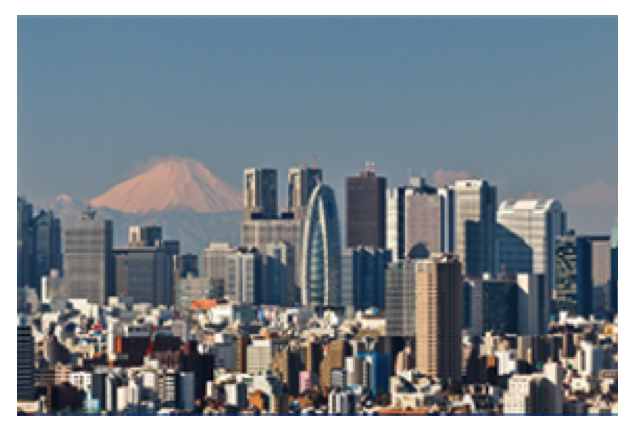
\includegraphics[width=60mm]{fig1.eps}
  \end{center}
  \caption{Figure caption.}
  \label{sample-figure}
\end{figure}

\subsection{Language}
All manuscripts must be in English.

\subsection{Formatting your paper}
Manuscript must be typed on A4-size papers---210 mm by 297 mm.
Print single-spaced text in two columns on each page. 
Text area should be adjusted to the following dimensions: 
top and bottom margins are both 25.4 mm; 
left and right margins are 18 mm; 
and column spacing is 8 mm. 
Fill each column from the top of the page except for the first page.

\subsection{Type-style and fonts}
Wherever Times is specified, Times New Roman may also be used. 
If neither is available on your PC, 
please use any available font that is closest in appearance to Times.

A manuscript should be formatted as follows:

\begin{description}

\item[Title:]
  The main title should be centered over 
  both columns and should be in Times 16-point, boldface type. 
  Capitalize the first letter of nouns, pronouns, verbs, 
  adjectives, and adverbs; do not capitalize articles, 
  coordinate conjunctions, or prepositions 
  (unless the title begins with such a word). 
  Long titles may be typed in two lines.

\item[Author Information:]
  Leave one blank line after the main title, 
  and then enter the full names of the authors, 
  followed by their affiliations. 
  Addresses and E-mail addresses help to contact authors. 
  Type in Times 12-point, non-boldface type. 
  Leave two blank lines after the author information. 
  {\it When you submit papers for review, please leave this area blank.}

\item[Abstract:]
  The abstract is typed in fully-justified text in 
  10-point italic, single-spaced, at the top of the 
  left-hand column, below the author and affiliation information. 
  Use the word ``{\bf Abstract}'' as the title, 
  in 12-point Times, boldface type, centered relative to the column, 
  initially capitalized. 
  The abstract is up to 200 words. 
  Leave at least one blank line after the abstract, 
  and then begin the main text.

\item[Section Heading and Text:]
  Text follows just after the abstract. 
  Type main text in 10-point Times, single-spaced. 
  Section headings should be Times 12-point boldface, 
  initially capitalized for each words, flush left. 
  Subsection headings should be Times 11-point boldface, 
  initially capitalized only for the first word. 

\item[Figures and Tables:]
  Figures and tables should be centered. 
  Figure caption should be centered, 10-point Times, 
  and placed below the figure. 
  Table caption should be typed as those for figures, 
  except it should be placed just above the table. 

\end{description}



\begin{table}[t]
  \caption{Table caption.}
  \begin{center}
    \begin{tabular}{c | c c c}
      \hline
      \hline
      \makebox[10mm]{Table} & \makebox[10mm]{1st} & 
      \makebox[10mm]{2nd} & \makebox[10mm]{3rd}\\
      \hline
      1 & 1.0 & 0   & 0 \\
      2 & 0   & 2.0 & 0 \\
      3 & 0   & 0   & 3.0 \\
      \hline
      \hline
    \end{tabular}
    \label{sample-table}
  \end{center}
\end{table}

\begin{figure}[t]
\noindent
Long captions should be set as in
  \begin{center}
    
\includegraphics[height=30mm]{fig2.eps}
  \end{center}
  \caption{
    This is an example of long caption requiring more than one line. 
    Long captions are placed beneath the figure with a 5 mm 
    additional margin on both sides.
  }
  \label{sample-figure2}
\end{figure}


\begin{description}

\item[Acknowledgments:]
  The acknowledgment section follows the main body. Please do not include acknowledgment before acceptance.
  
\item[References and Citations:]
  List and number all bibliographical references 
  in 9-point Times, single-spaced, at the end of your paper.
  When referenced in the text, enclose the citation number 
  in square brackets, for example\cite{IMR}. 
  Where appropriate, include the names of editors of referenced books.
  
\item[Appendices:]
  Appendices may follow the references. 
  Index appendices by letters or numbers in sequence, 
  and provide informative titles.

\end{description}


\balance

\section{Page Limits and Maximum File Size}
Page limit is 4 pages, excluding references, and papers should be printable on A4 paper. The submission file should not exceed 20 MB.


\section{Supplemental Materials}
Supplementary material (images, video, etc.) may optionally be submitted with
papers, but be sure to maintain anonymity, including the file properties or
other hidden text. The supplemental materials have a file size limit of 50
MB. The supplemental materials will not be part of the conference proceedings,
so they are only there to aid the reviewing process and award selecting
process. Reviewers are not required to view the supplemental material (though
most reviewers are likely to do so), so any information critical to
understanding the work should be in the main paper.

Note that all of the additional materials must be submitted as one pdf or zipped file.

\section{Producing and Testing PDF Files}
We recommend that you produce a PDF version of 
your submission well before the submission deadline. 
Besides making sure that you are able to produce a PDF, 
you will need to check that 
(a) the length of the paper remains within the page limit, 
(b) the file size is 20 MB or less, 
and (c) the file can be read and printed using Adobe Reader. 
Concerning (c), you must embed all necessary fonts into your PDF file. 
After embedding, check the file again according to 
the following procedure if you use Adobe Reader 9.5.1, for example.

\begin{itemize}
\item[(1)] Under the Edit menu, select ``Preferences''.
\item[(2)] In the Preferences dialog box under ``Categories'',
  select ``Page Display'', and then deselect ``Use Local fonts''.
\item[(3)] Under the File menu, select ``Properties''.
\item[(4)] In the Document Properties dialogue, select ``Fonts'' tab.
\item[(5)] Check whether all fonts are embedded properly.
\end{itemize}


\begin{thebibliography}{99}

\bibitem{IMR}
  I. M. Researcher, et al.: 
  ``Read My Excellent Paper,'' 
  \textit{Some Great Journal}, vol.xx, no.xx, pp.xx--xx, 200X.

\bibitem{MVA}
  MVA Conference: {\tt http://www.mva-org.jp/}

\bibitem{MVA2}
Anonymous, 202X.

\end{thebibliography}



\end{document}
